\section{Additional Implementation Details}\label{app:implement}

\subsection{Primitive Implementation}\label{app:implement_primitives}

\stitle{\textsf{CrossProduct}} $\crossproduct_{A_i,A_j\rightarrow A'}(\cdot)$: This primitive replaces the two attributes $A_i$ and $A_j$ by a single attribute $A'$. Given the encrypted input table $\encT$, where all attributes are in one-hot-encoding and encrypted, the attributes of $\encT$ except $A_i$ and $A_j$ remain the same. For every row in $\encT$, we denote the encrypted one-hot-encoding for $A_i$ and $A_j$ by $\tilde{\bf{v}}_1$ and $\tilde{\bf{v}}_2$.  Let $s_1$ and $s_2$ be the domain sizes of $A_i$ and $A_j$ respectively. Then the new one-hot-encoding for $A'$, denoted by $\tilde{\bf{v}}$, has a length of $s=s_1\cdot s_2$. For $l\in \{0,1,\ldots, s-1\}$, we have $$\tilde{\bf{v}}[l] = labMult(\tilde{\bf{v}}_1[l/s_2], \tilde{\bf{v}}_2[l\%s_2]).$$
Only one bit in $\tilde{\bf{v}}$ for $A'$ will be encrypted 1 and the others will be encrypted 0s. When merging more than two attributes, \system can use the $genLabMult()$ described in Section~\ref{genlab} to speed up computation.


%Let $D_1$ and $D_2$  be the encrypted one-hot-coding corresponding to two  values $v_1$ and $v_2$ (integral representation) for attributes $A_1$ and $A_2$ respectively. The corresponding encrypted one-hot-encoding for the two-dimensional attribute $A_1\times A_2$ is given by  \begin{gather} D_{1\times 2}[(i-1)\cdot s_{A_2}+j] = labMult(D_1[i], D_2[j])\\ i \in [s_{A_1}], j \in [s_{A_2}]\end{gather} For this particular case, only $D_{1 \times 2}[(v_1-1)\cdot s_{A_2}+v_2]=Enc(1)$ while all other indices will equate to $Enc(0)$. Note that when computing the one-hot-encoding for a t-dimensional attribute $t > 2$,  for the actual implementation, instead of calling $t$ iterative instances of \textsf{CrossProduct}() we use the $genLabMult()$ operator of labeled homomorphic encryption to speed up the computation.

\stitle{\textsf{Project}} $\project_{\bar{A}}(\cdot)$: The implementation of this primitive simply drops off all but the attributes in $\bar{A}$ from the input table $\encT$ and returns the truncated table $\encT'$.

\stitle{\textsf{Filter}} $\filter_{\phi}(\cdot)$: The predicate $\phi$ in this primitive is a conjunction of range conditions over $\bar{A}$, defined as: for a row $r$ in input table $\encT$,
$\phi(r) = \bigwedge_{A_j\in \bar{A}} ~~(r.{A_j} \in V_{A_j}),$ where $r.A_j$ is the value of attribute $A_j$ in row $r$ and $V_{A_j} \subseteq \{0,1,\ldots,s_{A_j}\}$ (the indices for attribute values of $A_{j}$ with domain size $s_{A_j}$).

First, we will show how to evaluate whether a row $r$ satisfies $r.{A_j} \in V_{A_j}$. Let $\tilde{\bf{v}}_j$ be the encrypted one-hot-encoding of $A_j$, then the indicator function can be computed as
$$I_{r.{A_j}\in V_{A_j}}=\bigoplus_{l\in V_{A_j}}\tilde{\bf{v}}_j[l].$$
If the attribute of $A_j$ in $r$ has a value in $V_{A_j}$, then $I_{r.{A_j}\in V_{A_j}}$ equals $1$; otherwise, $0$.

Next, we can multiply all the indicators using $genLabMult()$ (Section~\ref{genlab}) to check whether all attributes in $A_j\in \bar{A}$ of $r$ satisfy the conditions in $\phi$. Let $\bar{A} = \{A_1,\ldots,A_m\}$, then $$\phi(r) = genLabMult(I_{A_1\in V_{A_1}},\ldots, I_{A_m\in V_{A_m}}).$$

Last, we update the bit of $r$ in $\encB$, i.e., $\encB'[i] = labMult(\encB[i], \phi(r))$, given $r$ is the $i$th row in the input table. This step zeros out some additional records which were found to be extraneous by some preceding filter conditions.

Note that when the \textsf{Filter} transformation is applied for the very first time in a \system program and the input predicate is conditioned on a single attribute $A \in V_A$, we can directly compute the new bit vector using $I_{r.A\in V_{A}}$, i.e., for the $i$th record $r$ in input table $\encT$, we have $\encB'[i] =\bigoplus_{l\in V_A} \tilde{\bf{v}}_j[l]$.  This avoids the unnecessary multiplication $labMult(\encB[i],\phi(r))$.


%As discussed in the preceding section, the predicate $\phi$ is expressed in a special form of conjunctions of range conditions given by eq \ref{phi}. Now for a range condition $A \in \{v_1,...v_t\}$, assuming $\mathbf{\tilde{R}_A}[i]$ is the corresponding one-hot-coding for the $i^{th}$ record's value for attribute $A$,  consider the following \begin{gather}\mathbf{c}_A^i=\bigoplus_{j=1}^{t}\tilde{\mathbf{R}}_{A}[i][v_1]\end{gather} where $\tilde{\mathbf{R}}_{A}[i][v]$ is the $v^{th}$ index of corresponding one-hot-coding. Clearly if the $i^{th}$ record satisfies the condition $A \in \{v_1,...v_t\}$, then exactly one of the values in $\{\tilde{\mathbf{R}}_{A}[i][v_j]\}, j \in \{1,...,t\}$ will be a cipher for $1$. Thus $c_A^i=1$ if record $i$ satisfies the range condition and 0 otherwise. If the condition is instead an equality predicate $A==v$ then $\mathbf{c}_A^i=\tilde{\mathbf{R}}_{A}[i][v]$. Now considering $\phi$ is given by eq \ref{phi}, let us define\begin{gather}\mathbf{c}^i=genLabMult(\mathbf{c}^i_{A_1},...,\mathbf{c}^i_{A_r})\\A^*=\bigcup_{j=1}^rA_j\end{gather} It is easy to see that $c^i$=1 iff record $i$ satisfies $\phi$. Let $\mathbf{B}'$ be the indicator vector before the execution of the current instance of the \textsf{Filter} transformation. The final step is to multiply the $\mathbf{c}^i$s with the corresponding indicator bits and obtain the updated indicator vector $\mathbf{B}$ as follows \begin{gather}\mathbf{B}[i]=labMult(\mathbf{c}^i,\mathbf{B}'[i])\end{gather}
%The above step zeros out some additional records which were found to be extraneous by some preceding filter conditions. Clearly $\textbf{B}$ is the output of the \textsf{Filter} transformation.


%Avoid Indicator Vector Multiplication

%When the \textsf{Filter} transformation is applied for the very first time in a Crypt$\epsilon$ program and the input predicate is conditioned on a single attribute $A \in \{v_1,...,v_k\}$, then we can do the following optimization. Consider \begin{gather}\mathbf{b}[i]=\bigoplus_{j=1}^k \mathbf{\tilde{R}}_A[i][v_j], i \in [m]\end{gather} where $\mathbf{\tilde{R}}_A[i]$ is the one-hot-coding for attribute $A$ for the $i^{th}$ record. Since this is the first instance of the \textsf{Filter} primitive, the current indicator vector $\mathbf{B}$  will be all 1-vector. Thus $\mathbf{b}$ is itself the updated indicator vector  and we can avoid the unnecessary multiplication $labMult(\mathbf{b[i]},\mathbf{B}[i])$.

\stitle{\textsf{Count}} $\countagg(\cdot)$: To evaluate this primitive on its input table $\encT$, \system simply  adds up the bits in the corresponding $\encB$, i.e., $\bigoplus_{i}^m \encB[i]$.

%The \textsf{Count} primitive takes the associated bit vector $\mathbf{B}$ of its input table $\encT$  and simply adds up its entries to return  \begin{gather}\mathbf{c}=\bigoplus_{i=1}^m\mathbf{B}[i]\end{gather}%\item GroupBy*($\mathbf{V},sk$)- This primitive is an extension of the previous GroupBy transformation.

\stitle{\textsf{GroupBy*}} $\groupbystar_{A}(\cdot)$: The implementation steps for \textsf{Project}, \textsf{Filter} and \textsf{Count} are reused here. First, \system projects the input table $\encT$ on attribute $A$, i.e. $\encT_1 = \project_A(\encT)$. Then, \system loops each possible value of $A$. For each value $v$, \system initializes a temporary $\encB_v=\encB$ and filters $\encT'$ on $A=v$ to get an updated $\encB'_v$. Last, \system counts the number of 1s in $\encB'_v$ and release the counts.

\eat{
\begin{enumerate}[label=\alph*)] \item $\mathbf{\tilde{T}}_1$=\textsf{Project}($\mathbf{\tilde{T}}$, $A$) \item $\mathbf{B}$ =  current indicator bit vector \item  for $i = 1:s_A $ \\Intialize bit vector to $\mathbf{B}$  \\$\phi_i= (A==v_{i,A}) $ \\$\hat{\mathbf{T_2}}$ = \textsf{Filter}($\mathbf{\tilde{T}}_1, \phi_i$)\\ $\mathbf{C}[i]$ = \textsf{Count}($\hat{\mathbf{T_2}}$) \\ end for \item Output $\mathbf{C}$ 
\end{enumerate}
}

\stitle{\textsf{GroupByCount}} $\groupbystar_A(\cdot)$: The implementation detail of this primitive is given in the main text (section 5.2).

\stitle{\textsf{CountDistinct}}  $\countdistinct(\cdot)$: The implementation of this primitive involves both \AS and \CPS. Given the input encrypted vector of counts $\encV$ of length $s$, the AS first masks $\encV$ to form a new encrypted vector ${\bf \mathcal{V}}$ with a vector of random numbers $M$, i.e., for $i\in \{0,1,\ldots, s-1\}$,
${\bf \mathcal{V}}[i] = {\encV}[i] \oplus labEnc_{pk}(M[i]).$
This masked encrypted vector is then sent to \CPS and decrypted by \CPS to a plaintext vector $\mathcal{V}$ using the secret key.

Next, \CPS generates a garbled circuit which takes (i) the mask $M$ from the \AS, and (ii) the plaintext  masked vector $\mathcal{V}$ and a random number $r$  from the \CPS as the input. This circuit first removes the mask $M$ from $\mathcal{V}$ to get $V$ and then counts the number of non-zero entries in $V$, denoted by $c$. A masked count $c'=c+r$ is outputted by this circuit. \CPS send both the circuit and the encrypted random number $labEnc_{pk}(r)$  to \AS.

Last, the \AS evaluates this circuit to the masked count $c'$ and obtains the final output to this primitive: ${\bf c} = labEnc_{pk}(c') - labEnc_{pk}(r)$.

\eat{
   ($\mathbf{V},\epsilon$) - The \textsf{CountDistinct} primitive is implemented as follows \begin{enumerate}[label=\alph*)]\item Firstly the \textsf{AS} creates a mask vector drawn uniformly at random from $[m]^{s_A}$, i.e.,  \begin{gather*} M[i] \in_R [m], i \in [|V|]\end{gather*} \item \textsf{AS} masks the encrypted true count vector $\mathbf{V}$  as follows \begin{gather*}\boldsymbol{\mathcal{V}}[i]= \mathbf{V}[i] \oplus labEnc_{pk}(M[i])\end{gather*} and sends it to the \textsf{CSP} \item \textsf{CSP} decrypts the masked encrypted vector as \begin{gather*}\mathcal{V}[i]=labDec_{sk}(\mathbf{V}[i]), i \in [|V|]\end{gather*} \item Next the \textsf{CSP} generates the following garbled circuit that\begin{enumerate}[label=\roman*)]  \item takes the mask $M$ as an input from the \textsf{AS} \item takes a random number $r$  as an input from the \textsf{CSP}\item takes the decrypted masked vector $\mathcal{V}$ as an input from the \textsf{CSP} \item removes the mask $M$ from $\mathcal{V}$ as \begin{gather*}V[i]=\mathcal{V}[i]-M[i], i \in [|V|]\end{gather*}\item  counts the number of non-zero entries of $V$ as C \item adds the laplace noises \begin{gather*}\mathcal{C}=C+r\end{gather*} and returns $\mathcal{C}$ \end{enumerate} \item The \textsf{AS} evaluates the above circuit and gets output $\mathcal{C}$ \item The \textsf{AS} gets $labEnc_{pk}(r)$ from the \textsf{CSP} and generates $labEnc_{pk}(\mathcal{C})$ to compute\begin{gather*}\mathbf{C}=labEnc_{pk}(\mathcal{C})-labEnc_{pk}(r)\end{gather*} \end{enumerate}
}


\stitle{\textsf{Laplace}}  $\lap_{\epsilon,\Delta}(\mathbf{V})$:  The implementation of this primitive is presented in the main paper in sec 5.2.\eat{Given an encrypted vector counts $\encV$ of size $s$, both \AS and \CPS have to add Laplace noise in this primitive. Hence, this implementation involves two steps.

First, the \AS adds encrypted Laplace noise vector to $\encV$, i.e., for $i\in \{0,1,\ldots,s\}$, $\hat{\encV}[i]  = \encV[i] \oplus labEnc_{pk}(\eta_i),$ where $\eta_i\sim Lap(\Delta/\epsilon)$. This encrypted noisy vector $\hat{\encV}$ is then sent to the \CPS.

Next, the \CPS decrypts $\hat{\encV}$ using the secret key and add another Laplace noise vector, i.e., for  $i\in \{0,1,\ldots,s\}$, $\hat{V}[i] = labDec_{sk}(\hat{\encV}[i]) +\eta'_i$, where $\eta'~\sim Lap(\Delta/\epsilon)$. This plaintext noisy vector is returned as the final output of this primitive.}



\eat{
($\mathbf{V},\epsilon$)- Recall that both \textsf{AS} and \textsf{CSP} have to add Laplace noise to the output in Crypt$\epsilon$. Hence the \textsf{Laplace} primitive has two components. The first component is executed by the \textsf{AS} wherein,
\begin{enumerate} \item \textsf{AS} generates a noisy vector $\eta$ such that $\eta \in [Lap(\frac{1}{\epsilon})]^{|V|}$ \item encrypts $\eta$ and adds it to the input vector as \begin{gather*}\boldsymbol{\eta}=labEnc_{pk}(\eta)\\\mathbf{\hat{V}}[i]=\mathbf{V}[i]\oplus \boldsymbol{\eta}[i], i \in [|V|]\end{gather*} \end{enumerate} This encrypted noisy vector $\mathbf{\hat{V}}$ is the input for the second phase of the \textsf{Laplace} primitive which is executed by the \textsf{CSP} as follows \begin{enumerate}\item Decrypts $\mathbf{\hat{V}}$ \begin{gather*}\hat{V}=labDec_{sk}(\mathbf{\hat{V}})\end{gather*}  \item Generates a noisy vector $\eta'$ such that $\eta' \in [Lap(\frac{1}{\epsilon})]^{|\hat{V}|}$ \item Finally adds the noise $\eta'$ to $\hat{V}$ \begin{gather*}\hat{\mathcal{V}}[i]=\hat{V}[i]+\eta'[i], i \in [|\hat{V}|]\end{gather*} \item Returns $\hat{\mathcal{V}}$ to \textsf{AS} \end{enumerate} 
% Note that in the Crypt$\epsilon$ implementation we need to add two instances of the Laplace noise as opposed to a single instance in the standard central differential privacy setting. After the addition of the first instance of the laplace noise, $\eta$ (by the AS),  the encrypted answer is sent to the CSP. becuse of CSP has only a differential private view Hence the addition of the second instance of the laplace noise can be looked upon as a post-processing step  However and differential privacy is immune to post processing 
}


\stitle{\textsf{NoisyMax}} $\noisymax_{\epsilon,\Delta}^k(\cdot)$: The input to this primitive is an encrypted vector of counts $\encV$ of size $s$. Similar to \textsf{Laplace} primitive, both \AS and \CPS are involved. First,  the \AS adds to $\encV$
an encrypted Laplace noise vector and a mask $M$, i.e., for $i\in \{0,1,\ldots,s\}$,
$\hat{\encV}[i]  = \encV[i] \oplus labEnc_{pk}(\eta_i) \oplus M[i],$
where $\eta_i\sim Lap(\Delta/\epsilon)$. This encrypted noisy, masked vector $\hat{\encV}$ is then sent to the \CPS.

Next, the \CPS decrypts $\hat{\encV}$ using the secret key, i.e., for  $i\in \{0,1,\ldots,s\}$, $\hat{V}[i] = labDec_{sk}(\hat{\encV}[i])$. The \CPS generates a garbled circuit which takes  (i) the noisy, masked vector $\hat{V}$ from the \CPS, and (ii) the mask $M$ from the \AS as the input. This circuit will remove the mask from $\hat{V}$ to get the noisy counts $\hat{V}'$ and find the indices of the top-$k$ values in $\hat{V}'$.

Finally, the \AS evaluates the circuit above and returns the indices as the output of this primitive.


\eat{
($\mathbf{V},\epsilon,k$)- The input to the NoisyMax primitive is an encrypted vector $\mathbf{V}$ where each entry $V[i]$ is a count. The primitive is implemented via the following steps.  \begin{enumerate}
\item First the \textsf{AS} adds noise to the input encrypted vector as follows \begin{gather*} \eta \in [Lap(\frac{1}{\epsilon})]^{|V|}\\\boldsymbol{\eta}=labEnc_{pk}(\eta)\\\mathbf{\hat{{V}}}[i]=\mathbf{V}[i]+ \boldsymbol{\eta}[i], i \in [|V|] \end{gather*} \item Next the \textsf{AS} creates a mask vector $M$ drawn uniformly at random from $[m]^{s_A}$, i.e.,  \begin{gather*} M[i] \in_R [m], i \in [|V|]\end{gather*} \item \textsf{AS} masks the encrypted noisy vector $\mathbf{\hat{V}}$  as follows \begin{gather*}\boldsymbol{\mathcal{V}}[i]= \mathbf{\hat{V}}[i] \oplus labEnc_{pk}(M[i]), i \in [|V|]\end{gather*} and sends it to the \textsf{CSP} \item \textsf{CSP} decrypts the masked encrypted noisy vector as \begin{gather*}\mathcal{V}[i]=labDec_{sk}(\mathbf{\hat{V}}[i]), i \in [|V|]\end{gather*} \item Next, the following garbled circuit is evaluated which
    \begin{enumerate}[label=\roman*]\item takes noisy masked  vector $\mathcal{V}$ as an input from the \textsf{CSP} \item takes mask $M$ as the input from \textsf{AS}  \item removes the mask from  $\mathcal{V}$  as \begin{gather*} \hat{V}[i]=\mathcal{V}[i]-M[i], i \in [|V|]\end{gather*}  \item computes the top $k$ element over  $\hat{V}$ and returns $arg_{\textit{top k}}\max{\hat{V}[i])}$
    \end{enumerate}
    \end{enumerate}
}


\subsection{DP Index Optimization Implementation}\label{app:index-imp}

The DP index optimization can be implemented via a garbled circuit which aims to compute two pieces of information: a sorted encrypted database based on $A$ and a $\epsilon$-differentially private index on $A$. This circuit takes (i) the secret key $sk$ from the \CPS, and (ii) the entire database $\encD$ and the attribute $A$ from the \AS. The attribute $A$ has a domain of size $s_A$ and is uniformly partitioned into $k$ ranges $\{R_1,\ldots, R_i, \ldots, R_{s_A/k}\}$, where $R_i = [\frac{s_A}{k}i, \frac{s_A}{k}(i+1))$.

This circuit first decrypts $\encD$ using the secret key and sorts the decrypted database on attribute $A$ in ascending order. The sorted database is then encrypted again. Then the circuit computes a histogram $V$ on the $k$ ranges of $A$, denoted by $[c_1,\ldots,c_k]$  and perturbs each count with Laplace noise, i.e., $\hat{c}_i = c_i + \eta_i$, where $\eta_i\sim Lap(1/\epsilon)$. The noisy counts $\encV$ are then used to construct a cumulative histogram over $A$, where $\hat{cdf}[i] = \sum_{j=0}^i \hat{c}_i$ and post-processed such that they are in non-decreasing order and non-negative, and $\hat{cdf}[k] = |\encD|$~\cite{cdf}.

Given the differentially private cdf and the sorted database, when a program would like to select rows with $A\in [v_i, v_j]$, we find the ranges that contain $v_i$ and $v_j$ respectively, denoted by $R_i$ and $R_j$. Then we return all records in the sorted database which cover all ranges from $R_i$ and $R_j$. This corresponds to row $(\hat{cdf}[i-1]+1)$ to row $(\hat{cdf}[j])$.






\eat{
\begin{enumerate}\item takes the entire database $\boldsymbol{\mathcal{\tilde{D}}}$ as an input and the attribute $A$ as an input from the \textsf{AS}.
\item takes the secret key $sk$ as an input from  the \textsf{CSP} \item Decrypts $\boldsymbol{\mathcal{\tilde{D}}}$ \item Sorts the decrypted database on $A$, i.e., the first $ct_{A,v_1}$ rows are the ones with value $v_1$ for attribute $A$, the next $ct_{A,v_2}$ are  the records with value $v_2$ for attribute $A$ and so on. \item  re-encrypts the sorted database \item Divide the domain of $A$ into $k$ bins such that each bin contains $s_A/k$ consecutive domain values. \item Construct a $k$ lengthed vector $\hat{V}$ such that $\hat{V}[i]=\sum_jct_{A,j}+\eta_i, i \in [k], j \in [\frac{s_A}{k}(i-1)+1,\frac{s_A}{k}i]$ where $\eta_i$ is a random laplace noise drawn from the distribution $Lap(\frac{k}{\epsilon})$ \item Return $\hat{V}$ and sorted $\boldsymbol{\mathcal{\tilde{D}}}_{sort}$\end{enumerate}
}

\subsection{Illustration genLabMult}\label{app:genlabhe}
Figure~\ref{genlab-fig} illustrates how a $n$-way multiplication described in Section~\ref{genlab} can be parallelized. This approach requires a total of $\lceil \log n\rceil$ rounds of communication between \AS and \CPS.

\begin{figure}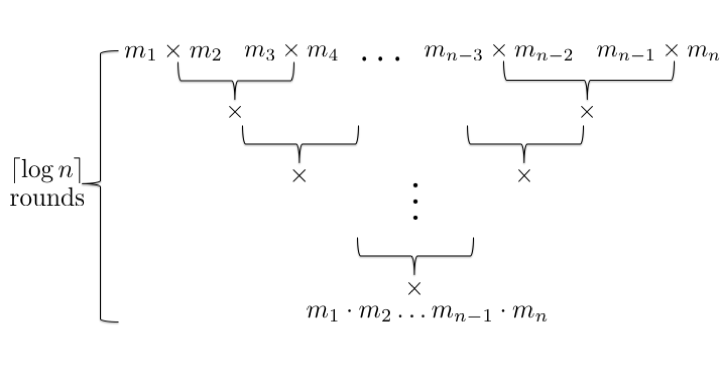
\includegraphics[width=\columnwidth]{kk.png} \caption{ $genLabMult()$ - Batching of multiplicands for \textsf{labHE}} \label{genlab-fig}\end{figure}
